\documentclass{article}
\usepackage{graphicx}
\usepackage{caption}
\graphicspath{ {./images/} }
 
\begin{document}
\paragraph{Basic HTTP Get/response interaction}
    \begin{enumerate}
      \item Is your browser running HTTP version 1.0 or 1.1? What version of HTTP is the server running?
        \begin{itemize}
          \item Browser: HTTPv1.1
          \item Server: HTTPv1.1
          \item 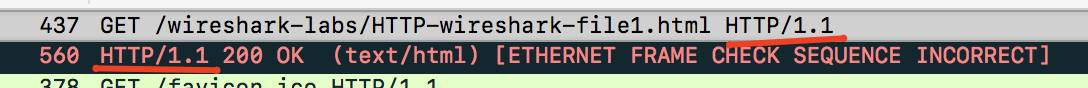
\includegraphics[scale=0.5]{images/HTTP1.png}
        \end{itemize}

      \item What languages does your browser indicate that it can accept to the server?
      \begin{itemize}
        \item My browser communicates that it can accept 'en-US'
        \item 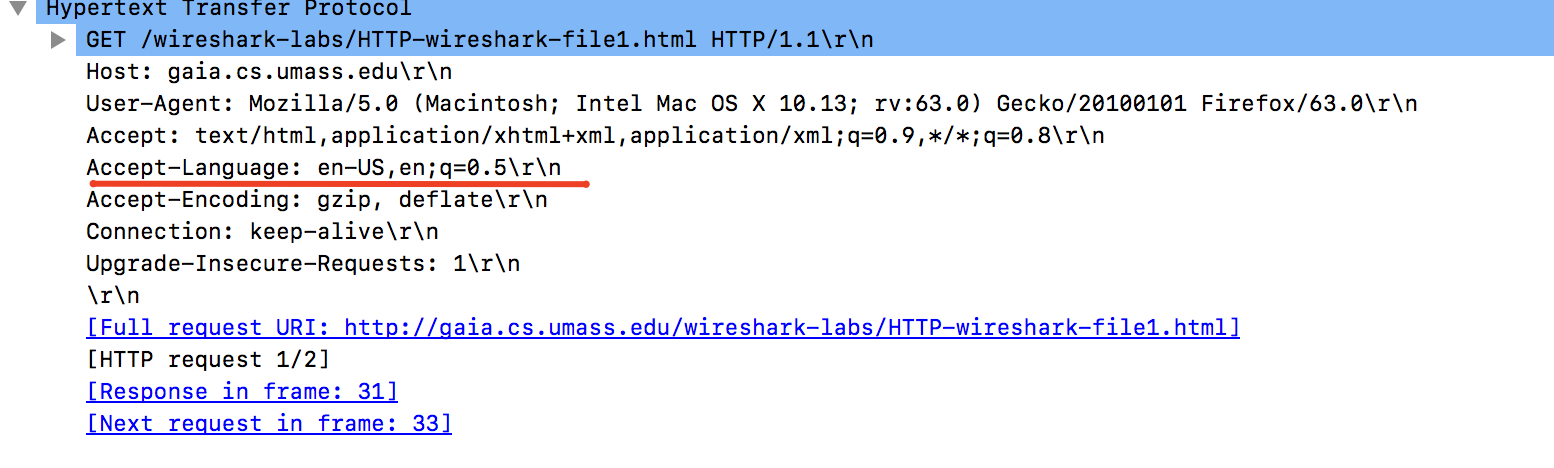
\includegraphics[scale=0.5]{images/HTTP2.png}
      \end{itemize}
      \item What is the IP address of your computer? Of the Server? 
        \begin{itemize}
          \item Me: 10.106.41.52
          \item Server: 128.119.245.12
          \item 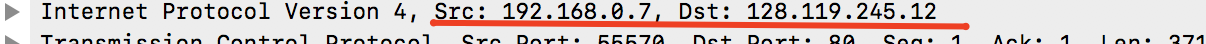
\includegraphics[scale=0.5]{images/HTTP3.png}
        \end{itemize}
      \item What is the status code returned from the server to your browser? 
        \begin{itemize}
          \item Status Code: 200 OK
          \item 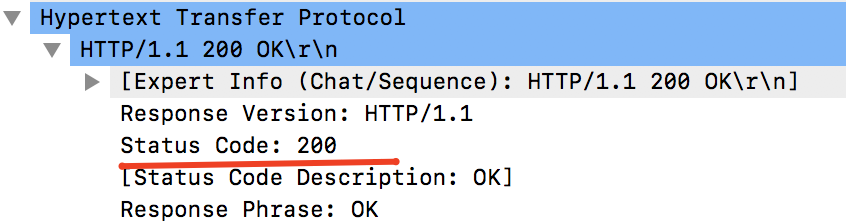
\includegraphics[scale=0.5]{images/HTTP4.png}
        \end{itemize}
      \item When was the HTML file that your are retrieving last modified at the server?
        \begin{itemize}
          \item Last Modified: THU, 08 Nov 2018 06:59:01 GMT
          \item 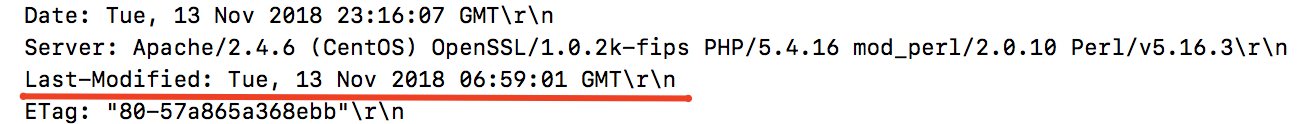
\includegraphics[scale=0.5]{images/HTTP5.png}
        \end{itemize}
      \item How many bytes of content are being returned to your browser?
        \begin{itemize}
          \item 128 Bytes
          \item 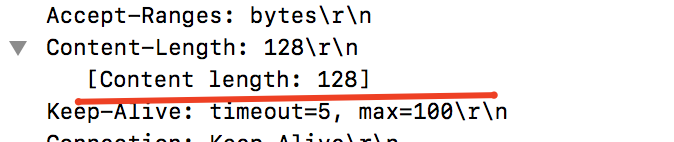
\includegraphics[scale=0.5]{images/HTTP6.png}
        \end{itemize}
      \item List a header not displayed in the packet listing:
        \begin{itemize}
          \item Connection: Keep Alive
        \end{itemize} 
    \end{enumerate}

  
  \paragraph{HTTP CONDITIONAL GET/response interaction}
  \begin{itemize}
    \item\begin{enumerate}
      \item Inspect the contents of the first HTTP GET reequest from your browser to the server.  Do you see an "IF-MODIFIED-SINCE" line in the HTTP GET? 
        \begin{itemize}
          \item No "IF-MODIFIED-SINCE" header in the first GET Request. 
        \end{itemize}
      \item Inspect the contents of the server response.  Did the server explicitly return the contents of the file? How can you tell?
      \begin{itemize}
        \item Yes, there was a content length field, and a specified number of bytes indicating the server explicitly downloaded the contents.
        \item 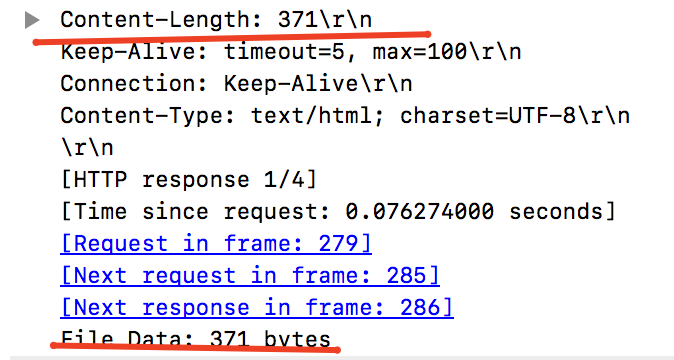
\includegraphics[scale=0.5]{images/HTTP9.png}
      \end{itemize}
      \item Now inspect the contents of the second HTTP GET request from your browser to the server.  Do you see an "IF-MODIFIED-SINCE:" header?
        \begin{itemize}
          \item There is an "IF-MODIFIED-SINCE" header in the HTTP GET request
          \item 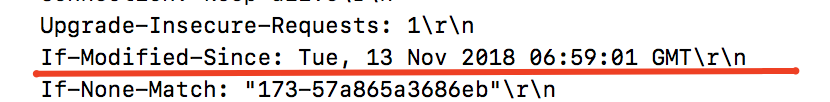
\includegraphics[scale=0.5]{images/HTTP10.png}
        \end{itemize}
      \item What is the HTTP status code and phrase returned form the server in response to this second HTTP GET? Did the server explicitly return the contents of the file? Explain.
        \begin{itemize}
          \item The HTTP status code is 304, not modified.
          \item The server returned a cached version of the file, there is no filedata field, and no amount of bytes specified.
          \item 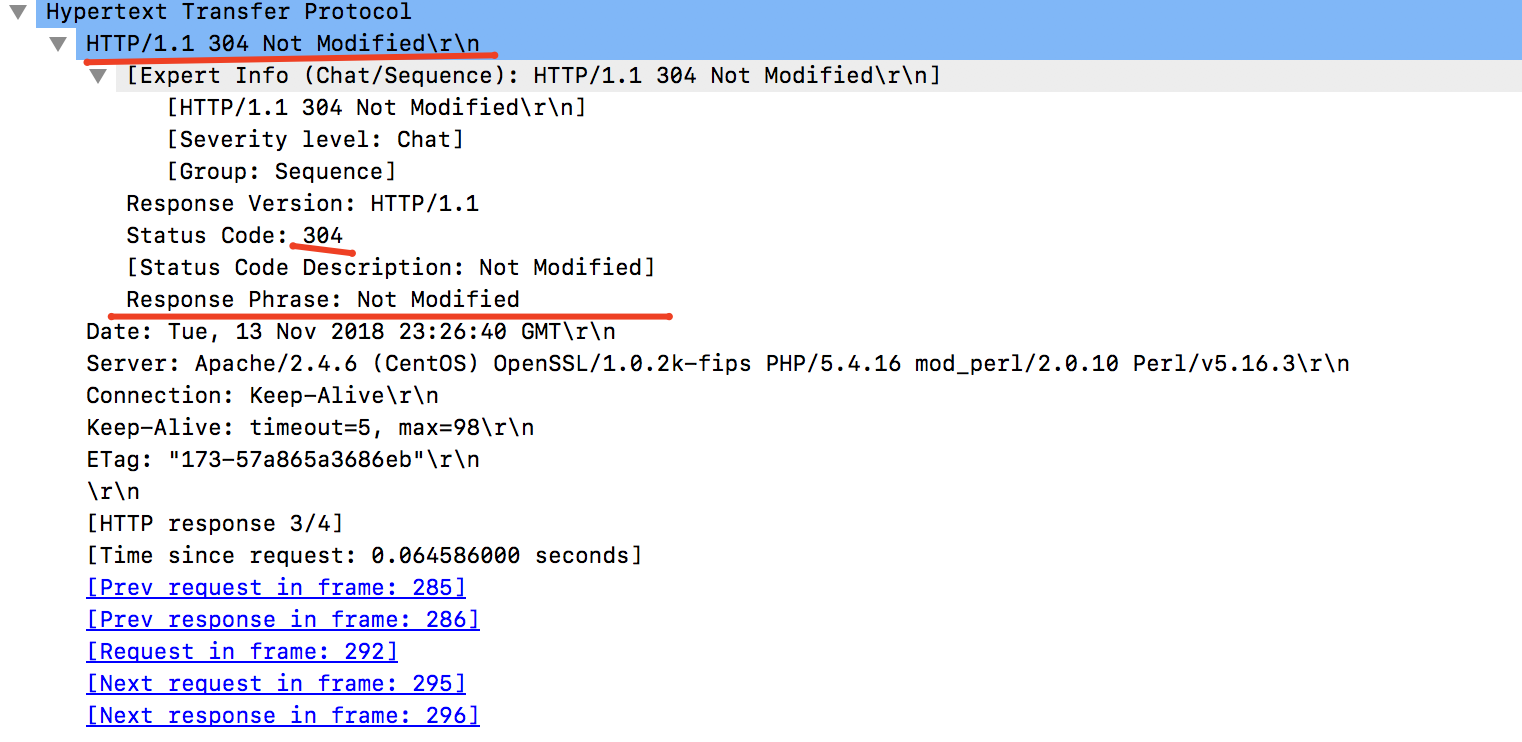
\includegraphics[scale=0.5]{images/HTTP11.png}
        \end{itemize}
    \end{enumerate}
  \end{itemize}



  \paragraph{Retrieving Long Documents}
  \begin{itemize}
    \item\begin{enumerate}
      \item How many HTTP GET request messages did your browser send? To which Internet addresses were these GET requests sent?
        \begin{itemize}
          \item There was 1 HTTP Get request sent
          \item Packet number 7 contains the GET message for the Bill of Rights
          \item 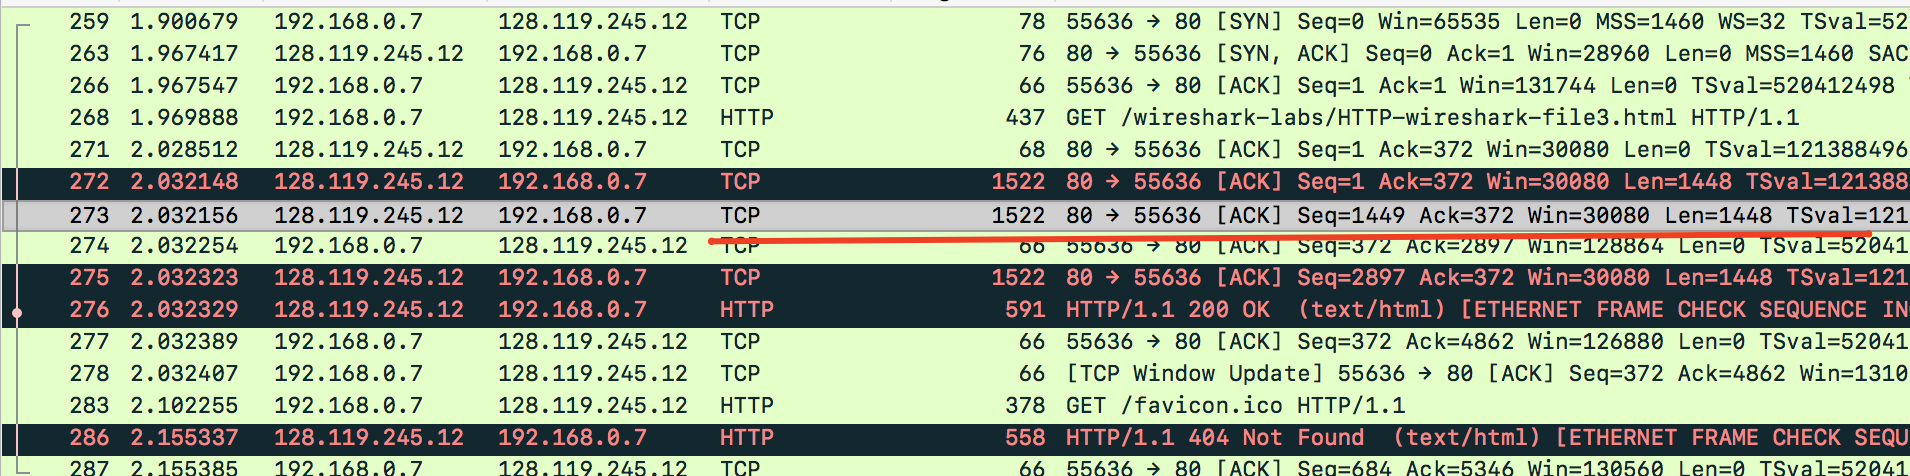
\includegraphics[scale=0.5]{images/HTTP12.png}
        \end{itemize}

      \item Which packet number in the trace contains the status code and phrase associated with the response to the HTTP GET request?
      \begin{itemize}
        \item the 4th Packet from the top (packet 268) in the trace contains the status code 
        \item 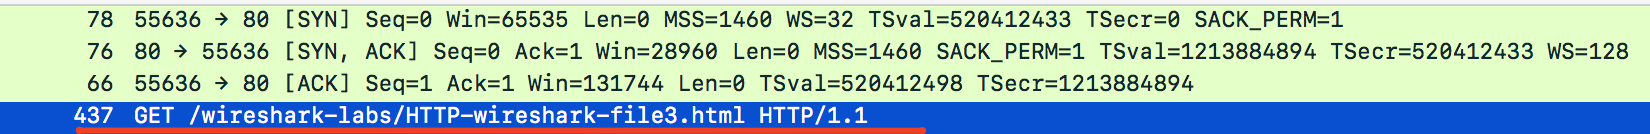
\includegraphics[scale=0.5]{images/HTTP13b.png}
      \end{itemize}
  
       \item What is the status code and phrase in the response?
          \begin{itemize}
            \item Status Code: 200
            \item Response Phrase: OK
            \item 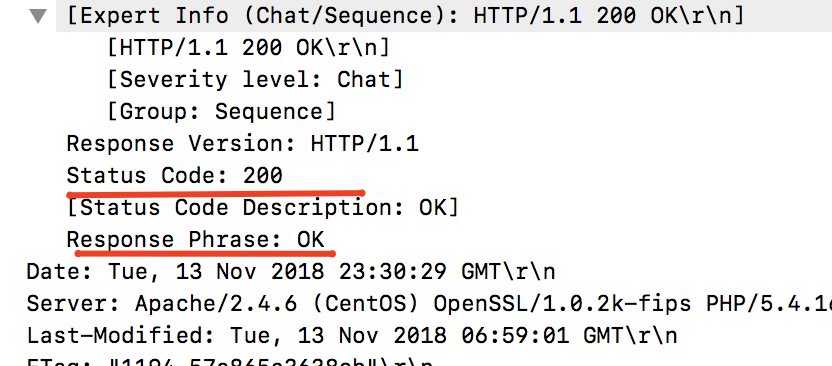
\includegraphics[scale=0.5]{images/HTTP15.png}
        \end{itemize}

      \item How many data-containing TCP segments were need to carry the single HTTP response and the text of the bill of rights?
        \begin{itemize}
          \item There are three packets that contain data for the Bill of Rights
          \item 271, 272, and 273
          \item 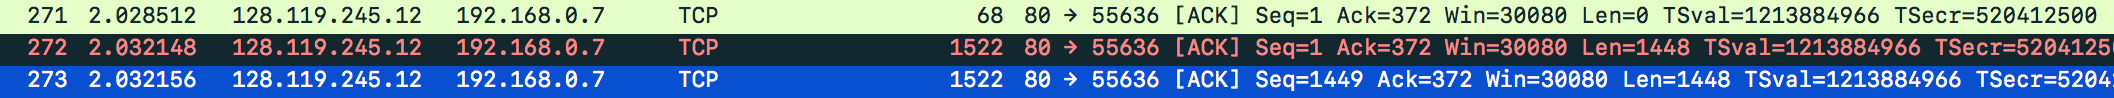
\includegraphics[scale=0.5]{HTTP15a.png}
        \end{itemize}
      \end{enumerate}

    \paragraph{HTML Documents with Embedded Objects}
    \begin{enumerate}
      \item How many HTTP GET request messaged did your browser send?  To which Internet Addresses were these GET requests sent?
      \begin{itemize}
        \item My browser sent three HTTP GET requests ignoring the favicon request
          \begin{enumerate}
            \item Packet 300 to 128.119.245.12 to download the Pearson.png
            \item Packet 301 to 128.119.245.12 to download the book cover
            \item Packet 307 to download the contents of the page
          \end{enumerate}
      \end{itemize}

      \item Can you tell whether your browser downloaded the two images serially, or whether they were downloaded from the two web sites in parallel?  Explain.
      \begin{itemize}
        \item The images were downloaded in parallel because processing of the request can't have finished before the next tcp request is opened, they are milliseconds apart as seen in the image
        \item 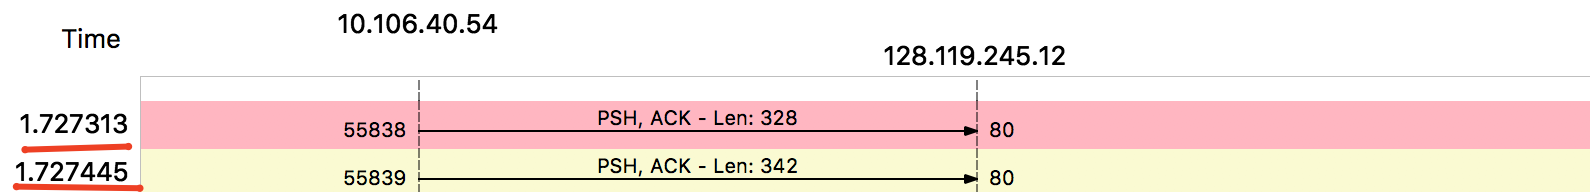
\includegraphics[scale=0.5]{images/HTTP18.png}
      \end{itemize}

  \end{enumerate}
  \end{itemize}

  \paragraph{HTTP Authentication}
  \begin{itemize}
    \item\begin{enumerate}
      \item What is the servers response in response to the initial HTTP GET message from your browser?
        \begin{itemize}
          \item Status Code: 401
          \item Phrase: Unauthorized
        \end{itemize}
      \item When your browser sends the HTTP GET message for the second time, what new field is included in the HTTP GET message?
          \begin{itemize}
            \item 'Authorization: Basic' is the new field included in the get request.
          \end{itemize}
    \end{enumerate}
  \end{itemize}

\end{document}
